\setcounter{chapter}{3}
\setcounter{rq}{1}


\chapter{Android Task Corpus}
\label{ch:android-corpus}



% ART: move to an early chapter
% To produce a solution for a task, a developer engages in a variety of
% information-seeking activities.  One of these activities involves
% the identification of  text in artifacts \gm{relevant to helping solve the task}.

Developing techniques that can automatically identify text
relevant to a task requires a means of evaluating whether
a proposed technique works well. In this context,
``working well'' refers to whether the text identified
by an automatic technique is similar to text considered
by humans as being relevant to a task at hand. To support
the evaluation of proposed techniques, a corpus
are needed that include tasks to be performed on
systems, artifacts representing different kinds of information
that would be useful to humans performing the tasks
and an identification of text in those artifacts that
is helpful to the humans.

As we have described earlier in this thesis, while there
exist techniques tuned to identifying relevant text in
specific artifact types, there are not techniques able to
identify text across a range of artifact types. Thus,
the corpa that exist consist of tasks with only single,
or a small number, of types of artifacts. As a result,
there was a need to create a corpa that included
multiple artifacts types for a task. This chapter describes the
development of a corpus that overcomes the limitations of
existing corpa, bringing together tasks from an existing
well-known domain, Android development, with relevant text
for solving that task from multiple artifact types.


Figure~\ref{fig:corpus-creation-pipeline}
summarizes the process we use to create the corpus, which we call \acs{DS-android}.
We randomly sample a set of 50 Android development tasks from two common
task sources, GitHub\footnote{\url{https://github.com/}} and Stack Overflow\footnote{\url{https://stackoverflow.com/}}.
For each of these tasks, we use the Google search engine to find potential artifacts that likely contain relevant
information for that task in top-ranked Android development websites. 
We then gather task-relevant sentences from these artifacts
from human experts.
We detail each of these steps in turn in 
Sections~\ref{cp4:corpus-tasks},~\ref{cp4:corpus-artifacts} and ~\ref{cp4:corpus-relevant-text}.
We provide a summary of the final created corpus in Section~\ref{cp4:corpus-summary}.




\gm{Pointer to how to get the corpus online right up front?}


\begin{figure}
    \centering
    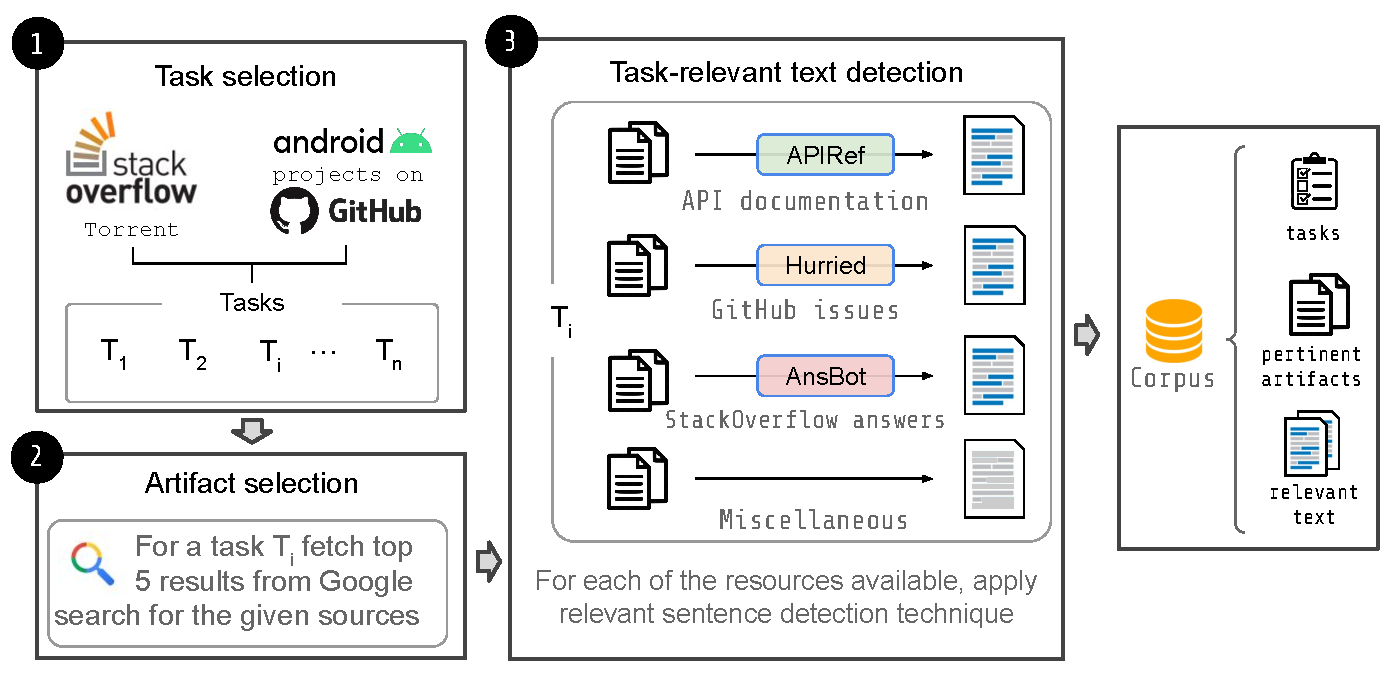
\includegraphics[width=1.05\textwidth]{cp4/corpus-creation-pipeline}
    \caption{Summary of procedures for corpus creation. \red{UPDATE}}
    \label{fig:corpus-creation-pipeline}
\end{figure}



\section{Software Tasks}
\label{cp4:corpus-tasks}

We start corpus creation by identifying software tasks 
for which a developer will likely benefit from 
the use of additional information to complete.
\rev{
We scope task selection to \textit{Android development} 
because the 
Android \acf{SDK} is always evolving due to 
functionality, security and performance-related improvements~\cite{Li2018android, Mateus2020}, what impact its development community and often require developers to seek information regarding changes in the SDK~\cite{linares2014, bavota2014b, mcdonnell2013}.
For example, over 35,000 developers have used Q\&A forums to discuss tasks covering 87\% of the classes in the Android API~\cite{parnin2012}.}


Two common places where Android task can be found are:


\begin{itemize}
    \item the description of an issue
    (e.g., a bug or feature request) reported in an issue tracking system; or in
    \item a post in a community forum, development mailing lists, and others.
\end{itemize}

Several studies have used such sources for software tasks~\cite{Arya2019, baltes2019, nadi2020, Xu2017}
and, following the lead
of these studies, we select GitHub issues and \acf{SO} posts on Android development as 
the two sources for the tasks in our corpus.



\subsubsection{GitHub tasks}

To select tasks from GitHub, we are guided by studies that use 
stars~\cite{borges2016, borges2018}
as a proxy for a project's popularity~\cite{Ferreira2016, Xavier2020}.
We selected 14 projects,
ranging from mail clients\footnote{\url{https://github.com/k9mail/k-9}}
to development frameworks\footnote{\url{https://github.com/libgdx/libgdx}},
by filtering the list of top-starred projects in GitHub to those with the \textit{Java} and \textit{Android} tags.
\rev{We then randomly selected 25 distinct issues originating from these starred projects as the GitHub tasks of our corpus (average of 1.78 issues per project).}
%  with an average of 1.78 issues per project
% For each of these projects, we randomly select 10 issues as the GitHub tasks of our corpus for a total of 150 distinct issues.
While selecting issues, we took care to check that they had at least one follow-up comment and that the issue title did not contain certain words, e.g., {\small \texttt{test}} or {\small  \texttt{ignore}},
as these words indicate issues  created automatically by scripts or bots---a common pitfall that researchers must be aware of when mining GitHub~\cite{kalliamvakou2014}.


Figure~\ref{fig:lock-screen-task} shows an example of a GitHub task in our corpus.
Although the expected behaviour is that the app controls should be visible even with the screen locked,  a user reports that the app screen is missing.
A developer addressing this issue might need to review the Android lock task documentation~\cite{apiLockTask}
or refer to examples of applications that use the Android lock screen~\cite{mediumLockApp}.
For the remainder of this chapter, we use the lock screen task as a running example.


\begin{figure}
    \centering
    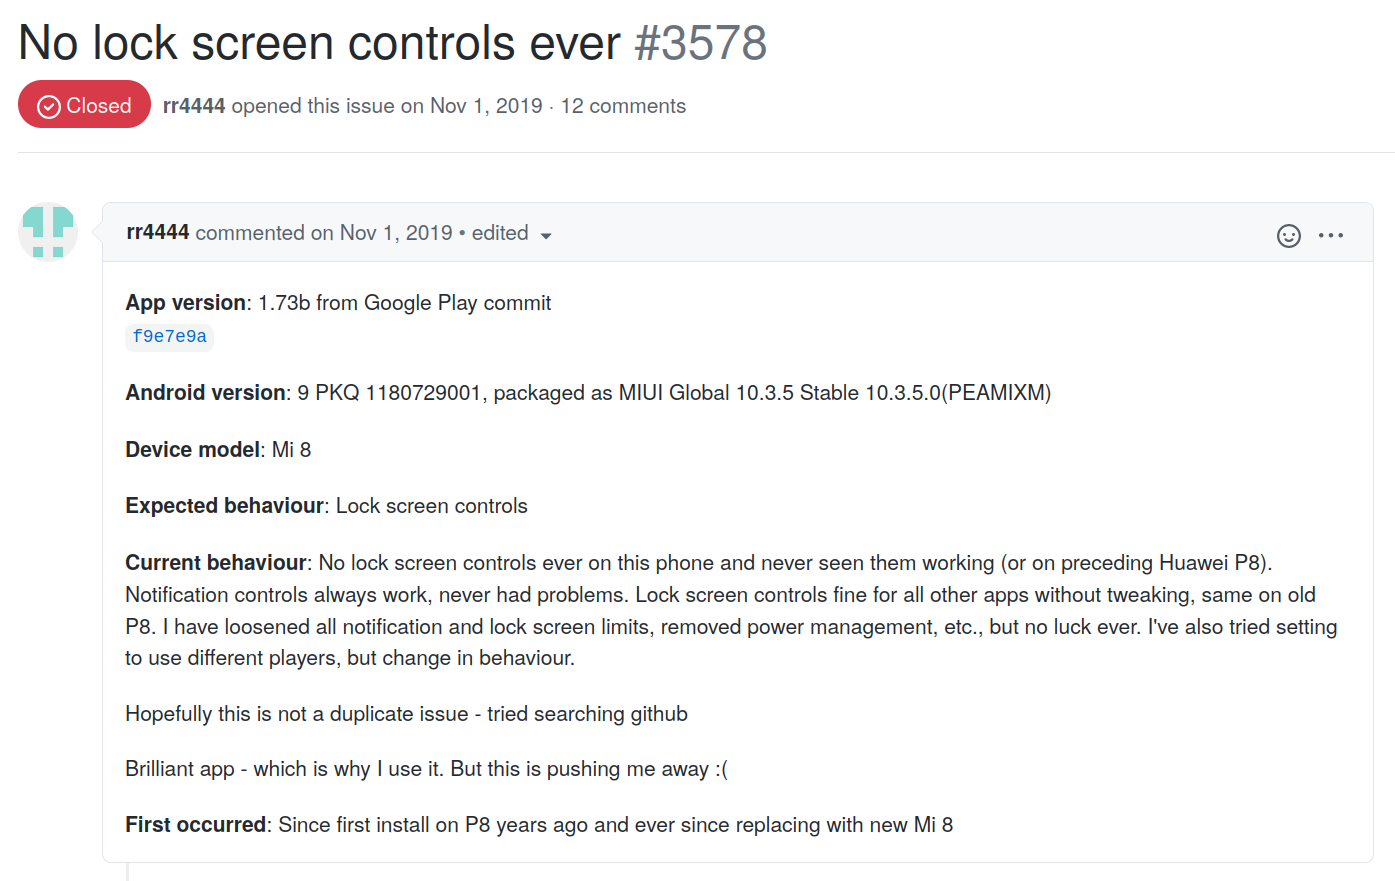
\includegraphics[width=\textwidth]{cp4/lock-screen-task}
    \caption{Sample GitHub task from our corpus}
    \label{fig:lock-screen-task}
\end{figure}



\subsubsection{Stack Overflow tasks}

%Provided that we restrict our corpus to tasks related to %the Android development domain,


We consider Stack Overflow posts as software tasks because to answer a post,
a developer often needs to provide references
supporting their answer~\cite{yazdaninia2021}.
Finding these references in a timely manner and writing the key information that helps a user understand 
 the provided solution encompasses many of the activities found in a developer's daily work, e.g., work-related browsing, coding, debugging, and reading/writing documentation~\cite{Meyer2017}.
For example, Figure~\ref{fig:webview-task} depicts a task where a developer describes her struggles using the Android WebView component.
To answer this question, a developer will not only provide a code snippet, but also explain key points of the Android Webview API~\cite{apiWebView}
and how they were used in the solution provided to the task, 
as presented in Figure~\ref{fig:webview-task-answer}.


\begin{figure}
    \centering
    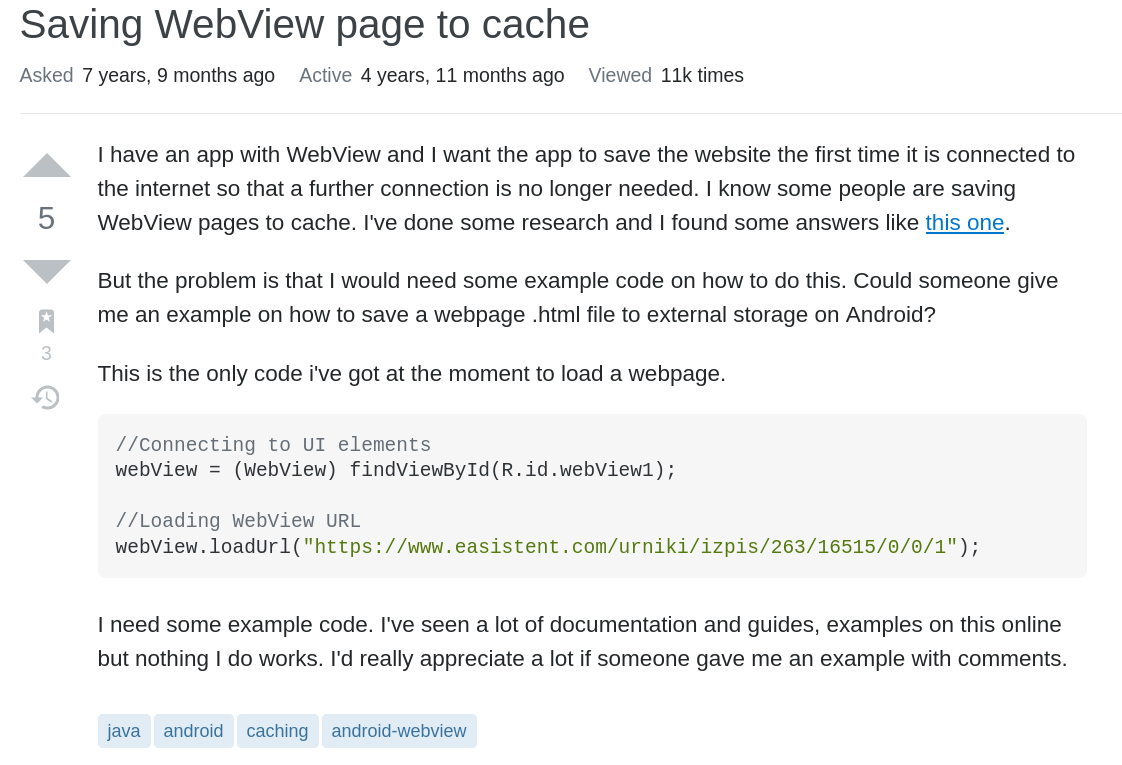
\includegraphics[width=0.85\textwidth]{cp4/webview-task}
    \caption{Sample Stack Overflow question}
    \label{fig:webview-task}
\end{figure}



\begin{figure}
    \centering
    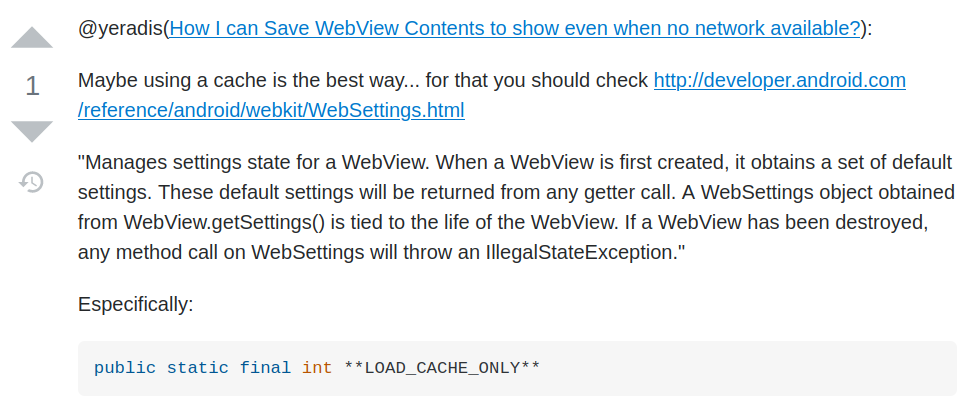
\includegraphics[width=0.85\textwidth]{cp4/webview-task-answer}
    \caption{Excerpt of a Stack Overflow answer}
    \label{fig:webview-task-answer}
\end{figure}

We randomly select \rev{25} Stack Overflow posts from a curated list about Android development~\cite{baltes2020}.
This list was built by Baltes et al. 
using the Stack Overflow dump published on June 5, 2018~\cite{baltes2019-rep, SOTorrent2019}
and it contains 209,536 unique posts with the \textit{Java} and \textit{Android} tags.



% When selecting tasks in GitHub and Stack Overflow, a major challenge arises due to the sheer amount of data available.
% Baltes et al.~\cite{baltes2019} argues that even a cursory inspection of a sample set
% of Stack Overflow posts shows clear differences in a post's content or structure due to aspects such as programming languages, frameworks, associated technologies, and others.
% \gm{-It feels like there is a missing sentence about how differences relate
% to the 'sheer amount of data' and why the differences matter.}

% To ensure the tasks in the corpus we produce
% circumvent \gm{-circumvent has a negative connotation - is there a way
% to say this positively?} the heterogeneity of data on GitHub and Stack Overflow, we scope task selection to the \textit{Android} development domain. This decision
% restricts task selection to a single programming language (\textit{Java})
% while still enabling investigation of a domain that has been
% widely discussed by practitioners and researchers alike.



\section{Artifact Selection}
\label{cp4:corpus-artifacts}


When selecting artifacts pertinent to a task in our corpus, we seek to simulate everyday practices on how developers search the Web~\cite{rao2020, Xia2017}.
We formulate a query for each task and use a Web search engine to retrieve artifacts that are pertinent to that task, as described below.


\subsubsection{Artifact sources}



The artifacts sought to find useful information or knowledge for completing a task
 depend on the type of task a developer performs.
For example, when using a new framework or library, a developer refers to official API documentation~\cite{Li2013,robillard2011field} while, for debugging or error diagnostic tasks, community-based sources are preferred~\cite{Li2013,Breu2010}.
Despite such variability, researchers have observed that Web blogs, API documentation, and community forums are sources
commonly used by developer to forage information that assists task completion~\cite{Li2013, josyula2018}.



We use this knowledge to restrict artifact selection to well-known and studied artifact types within these sources~\cite{Starke2009,Kevic2014, Li2013}, namely Android and Java SE API documentation, GitHub issues, Stack Overflow answers, and Web tutorials or blog posts on Java and Android development.





\subsubsection{Query formulation}



Coming up with proper search terms is a critical step of any search~\cite{Haiduc2013}
and, ideally, we should be able to formulate a query with terms able to retrieve the most pertinent artifacts for a software task.
However, studies have shown that developers perform poorly in identifying good search terms~\cite{latoza2006, Starke2009,Kevic2014} and thus, using a task's title
as an educated approximation to terms that a developer might use is a common procedure adopted by other studies in the field (e.g.,~\cite{Xu2017} or ~\cite{silva2019}).
Hence, we use a task's title (i.e., SO question or GitHub issue title) as the seed to search for pertinent artifacts.



\subsubsection{Search results}


We use \texttt{googlesearch} API~\cite{googlesearch} to 
request up to 5 resources per query
adding \texttt{site:domain} to search for artifacts 
only in (or outside) a given web domain\footnote{e.g., \texttt{site:stackoverflow.com} for a query searching for Stack Overflow artifacts}---procedures similar to~\cite{Xu2017}.



From the results returned, we include up to
one API document, one GitHub issue discussion, one Stack Overflow answer, and two miscellaneous web pages
in the final artifact set for a task. 
When selecting results, we exclude any entry that does not appear in the Amazon Alexa~\cite{alexa} web traffic statistics for Java and Android development in the period from April 2020 to March 2021. 
We apply this filter to include software development artifacts and remove results 
such as a tutorial about  ``\textit{stock swap}'' operations which was initially fetched 
for a task discussing ``\textit{left and right-hand swap}''.
Table~\ref{tbl:googlesearch-example-git} shows one search result per artifact source for the GitHub task introduced in Section~\ref{cp4:corpus-tasks}


Limiting the number of artifacts up to a maximum of 5 artifacts per task relates to the
time-consuming~\cite{al2017} and cognitively demanding~\cite{Piorkowski2016} 
nature the final step in the dataset creation, i.e.,  
asking annotators to carefully read, understand and identify the text
within the fetched artifacts that relevant to a given task,
as Section~\ref{cp4:corpus-relevant-text} further details.





\begin{table}[H]
\centering    
\begin{scriptsize}
\begin{threeparttable}
\rowcolors{2}{}{lightgray}    
\begin{tabular}{l|l}

\hline

\multicolumn{2}{c}{\textit{Saving WebView page to cache}}  \\

\hline
\hline

\multirow{1}{*}{API documentation}
& Managing WebView objects - Android Developers \\
% & WebView - Android Developers \\

\multirow{1}{*}{Github issues}
& WebView Caching contents WebView using the cachePolicy \\
% & Investigate whether removing WebView files on erase is a good idea \\


\multirow{1}{*}{StackOverflow answers}
& Android WebView not loading second page from cache \\
% & Save webview content for offline browsing? \\
\hline

\end{tabular}
\end{threeparttable}
\end{scriptsize}
\caption{Sample of artifacts obtained for a StackOverflow task~\cite{so18607655}}
\label{tbl:googlesearch-example-so}
\end{table}



\begin{table}[H]
\centering    
\begin{scriptsize}
\begin{threeparttable}
\rowcolors{2}{}{lightgray}    
\begin{tabular}{l|l}

\hline

\multicolumn{2}{c}{\textit{No lock screen controls ever}}  \\

\hline
\hline

\multirow{1}{*}{API documentation}
& Lock task mode - Android Developers \\
% & Recents Screen - Android Developers \\

\multirow{1}{*}{Github issues}
& Lock screen controls disappear on Android 11 \\
% & Bug: No lock screen image and controls \\


\multirow{1}{*}{StackOverflow answers}
& How to add MediaPlayer controls on lock screen? \\
% & How to disable home button in Android like lock screen apps do? \\



\multirow{1}{*}{Miscellaneous}
& Create A React Native App - Which works on Lock Screen (Android) \\

\hline


\end{tabular}
\end{threeparttable}
\end{scriptsize}
\caption{Sample of artifacts obtained for a Github task~\cite{git3578} }
\label{tbl:googlesearch-example-git}
\end{table}



\subsubsection{Artifact's content}

Last, we need to extract the natural language text within an artifact so that 
techniques that automate the identification of text relevant to a task can be built 
using our corpus.  This step requires processing an artifact's content 
into a sequence of individual sentences,
what prompted us to follow common procedures for processing the artifact types found in our corpus~\cite{Arya2019, nadi2020}.
That is, given a search result \texttt{URL}, we use use a series of python 
APIs\footnote{\texttt{BeautifulSoup}~\cite{beautifulsoup4},
\texttt{StackAPI}~\cite{StackAPI} and \texttt{PyGithub}~\cite{PyGithub}}
to fetch the artifacts' content
and then, we use the Stanford CoreNLP toolkit~\cite{CoreNLP} to identify 
individual sentences in the artifacts' content.












\section{Relevant text detection}
\label{cp4:corpus-relevant-text}






Next, we need to determine which 
of the text in the gathered artifacts could provide information that assists a developer in solving her task.
In our corpus, this text represents \textit{golden data} that one can use to design and evaluate automatic tools that assist developers in the identification of information useful to their tasks. 
To produce it, we 
ask experienced developers to
mark the text that they deem useful and that provide information for tasks assigned to them~\cite{nadi2020, Robillard2015, marques2020}.



\subsection{Annotation process}


Our intention is that golden data reflect text that instructs developers to perform important actions to accomplish their task~\cite{Robillard2015, Lotufo2012}.
To this end, we describe the annotators' background, annotation procedures, and the 
the text inspected by the annotators.
% FIXME: find a way to format the standard deviation acronym
\textcolor{white}{\acs{stdv}} % force acronym to appear in the glossary for the time being





\subsubsection{Annotators}


We recruited 3 graduate students with professional programming experience to produce \textit{golden} data for our corpus. Annotators had to have experience with Java development and they also had to be familiar with the types of artifacts they would encounter throughout the annotation process. 
On average, annotators self-reported 3.0 years of professional
programming experience (stdv 1.63, ranging from 1 to 5 years).



\subsubsection{Annotation procedures}



We divided tasks into batches of 10 tasks each as to avoid fatigue effects~\cite{Ponzanelli2017}. For each batch, annotators had task descriptions and links to artifacts pertinent to the respective task at their disposal. We asked annotators to write a short plan (250 words max~\cite{Rastkar2010}) with instructions that a developer could follow to complete the task successfully. 
The purpose of the plan was to ensure that annotators built enough context about the task.
While perusing artifacts, annotators also had to manually highlight sentences that they deemed useful and that provided information that assisted task completion---instructions similar to the ones used for the creation of the data in the \acs{DS-synthetic} corpus~\cite{marques2020}.


The annotation process was facilitated by a tool we created for this purpose. Figure~\ref{fig:corpus-annotation-tool} shows a screenshot from the tool in 
action, which works as a browser plug-in. The top-right corner panel in the figure shows the browser extension. When an annotator clicked the \texttt{highlight} button, 
the tool instrumented the HTML of a page identifying individual sentences. The tool then allowed annotators to hover over identified sentences and to select them as relevant by clicking on the hovered text. For example, in the first paragraph, an annotator selected  the sentence
``\textit{Call ActivityOptions.setLockTaskEnabled() ... when starting the activity}'' as relevant to the Android lock task (Figure~\ref{fig:lock-screen-task}).







\begin{figure}
    \centering
    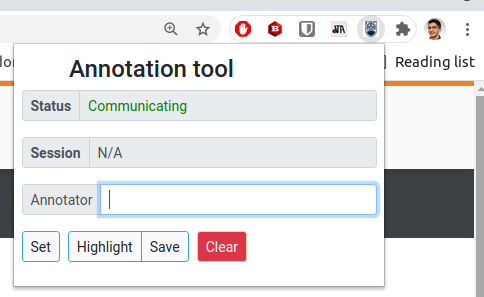
\includegraphics[width=\textwidth]{cp4/annotation-tool}
    \caption{Annotation tool and relevant sentences marked by an annotator}
    \label{fig:corpus-annotation-tool}
\end{figure}




\subsubsection{Text inspected}





Annotators had to inspect a total of 12,401 sentences originating from API documentation, Stack Overflow answers, GitHub issue discussion and miscellaneous Web pages.
These sentences comprise natural language written text---in this case, English---and do not involve source code snippets that may appear alongside the text.


Table~\ref{tbl:corpus-summary} gives insight into the number of sentences inspected per artifact type. 
We observe that API documents and miscellaneous Web pages contain the highest number of sentences in our corpus.
This is not surprising because API documents often contain boilerplate text 
and all the information needed for the usage of an API element is usually found in a single document~\cite{robillard2011field}.
Miscellaneous Web pages comprise blogs or tutorials, 
which often provide step-by-step instructions and accompanying examples, 
what likely explains the large number of sentences for this type of artifact~\cite{arya2020, Jiang2016b}.


The content of GitHub issues mostly resembles conversations~\cite{Rastkar2010}
and, beyond code snippets and minimal structured fields, the 
1,890 sentences inspected in this type of artifact comprise the description of a reported bug or a feature request as well as questions, answers, and discussion from  community members who are interested in resolving the issue at hand~\cite{zimmermann2010}.



For SO answers, the fewer number of inspected sentences (1,420) potentially relates to 
the fact that Stack Overflow offers little incentive for further discussion once a post has been answered.
Nonetheless, it is worthy noting that sentences with crucial information 
are not limited to the ones in an accepted answer~\cite{nadi2020}
and that later comments can be equally or more informative,
often providing notes about updates in an API component or framework~\cite{zhang2019so}.




\begin{table}[!h]
\centering    
\begin{small}
\begin{threeparttable}
\begin{tabular}{lccc}





& \multicolumn{3}{c}{\textbf{\# of sentences}}
\\ \cmidrule(l){2-4} 
& total & mean & stdv  \\

\hline
\hline

\textbf{API documentation} 
& 4,915 & 109.22 & 96.77
\\
\textbf{GitHub issues} 
& 1,890 &  43.95 & 33.69
\\
\textbf{SO answers} 
& 1,420 & 28.40 & 28.48 
\\
\textbf{Miscellaneous Web pages} 
& 4,176 & 70.78 & 56.64 
\\

\hline
\hline
\textbf{Overall} 
& 12,401 & 62.95 & 66.25 
\\
\hline

\end{tabular}
\end{threeparttable}
\end{small}
\caption{Summary statistics for the \acs{DS-android} corpus}
\label{tbl:corpus-summary}
\end{table}






\subsection{Corpus Description}

% \gm{The important point here is what
% is in the corpus - all sentences marked by annotators and who marked which?}


% \gm{Need to move table up so it is Table 4.3} -- OK
We structure tasks and annotation results in a format similar to the one shown in 
Table~\ref{tbl:corpus-data-structure}. 
Each task has a  title, link, description, and a set of pertinent artifacts.
In turn, each artifact has a type, title, link, and content,
where each sentence within an artifact's content
is preceded by the set of 
annotators (i.e., \texttt{none}, \texttt{A1}, \texttt{A2}, or \texttt{A3}) who marked the sentence as useful to the task.
As an example, in a Stack Overflow answer (artifact$_2$), all three annotators 
marked the sentence ``\textit{Have you checked RemoteControlClient?}''
as relevant to the lock mode task.

Overall, annotation required a total of $\approx60$ hours of manual work and it was done throughout the course of 4 weeks.
Table~\ref{tbl:corpus-annotation-summary} provides summary statistics for the text marked by 
the annotators over all the artifacts inspected as well as on an artifact type basis.





\clearpage

\begin{landscape}
\begin{table}
\begin{scriptsize}
% \vspace{-3mm}        
\begin{tabular}{cl}
\multicolumn{2}{l}{\cellcolor{lightgray}
    \textbf{Task}
}
\\
\multicolumn{2}{l}{\hspace{3mm}
\parbox[l][0.7cm][c]{16cm}{
    \texttt{No lock screen controls ever
}}}
\href{https://github.com/AntennaPod/AntennaPod/issues/3578}{link}
\\
\multicolumn{2}{l}{\cellcolor{lightgray}
    \textbf{Description}
}
\\
\multicolumn{2}{l}{
\hspace{3mm}
\parbox[l][2.5cm][c]{21cm}{
{\ttfamily
    \ldots
    \\
    \textbf{Expected behaviour:} Lock screen controls
    \\
    \textbf{Current behaviour:} No lock screen controls ever on this phone and never seen them working (or on preceding Huawei P8). Notification controls always work, never had problems. Lock screen controls fine for all other apps without tweaking, same on old P8. I have loosened all notification and lock screen limits, removed power management, etc., but no luck ever. I've also tried setting to use different players, but change in behaviour. \ldots
}}}
% --------------------------------------------------------------------------------------------------
\\
\hline
\hline
\multicolumn{2}{l}{\cellcolor{lightgray}
    \textbf{Artifact}$_1$ - \textbf{API documentation}}
\\
\multicolumn{2}{l}{\hspace{3mm}
\parbox[l][0.7cm][c]{16cm}{
    \texttt{Lock task mode Android Developers
}}}
\href{https://developer.android.com/work/dpc/dedicated-devices/lock-task-mode}{link}
\\
\multicolumn{2}{l}{\cellcolor{lightgray}
    \textbf{Content}}
\\
\texttt{none} & 
\parbox[l][0.6cm][c]{20cm}{
{\ttfamily    
    Android can run tasks in an immersive, kiosk-like fashion called lock task mode.
}}
\\
\texttt{A1} & 
\parbox[l][0.6cm][c]{20cm}{
{\ttfamily    
    Only apps that have been allowlisted by a device policy controller (DPC) can run when the system is in lock task mode.
}} 
\\
\texttt{none} & 
\parbox[l][0.6cm][c]{20cm}{
{\ttfamily    
    A DPC must allowlist apps before they can be used in lock task mode. 
}} 
\\
\texttt{A1, A2} & 
\parbox[l][0.6cm][c]{20cm}{
{\ttfamily    
    Call DevicePolicyManager.setLockTaskPackages() to allowlist apps for lock task mode as shown in the following sample
}} 
\\
\multicolumn{2}{c}{\texttt{...}}
% --------------------------------------------------------------------------------------------------
\\
\hline
\hline
\multicolumn{2}{l}{\cellcolor{lightgray}
    \textbf{Artifact}$_2$ - \textbf{Stack Overflow answer}}
\\
\multicolumn{2}{l}{\hspace{3mm}
\parbox[l][0.7cm][c]{16cm}{
    \texttt{Media Control on Lock Screen like Google Play Music in android?
}}}
\href{https://stackoverflow.com/questions/24652078/media-control-on-lock-screen-like-google-play-music-in-android}{link}
\\
\multicolumn{2}{l}{\cellcolor{lightgray}
    \textbf{Content}}
\\
\texttt{A1, A2, A3} & 
\parbox[l][0.6cm][c]{20cm}{
{\ttfamily    
Have you checked RemoteControlClient? 
}}
\\
\texttt{A2, A3} & 
\parbox[l][0.6cm][c]{20cm}{
{\ttfamily    
    it is used for the Android Music Remote control even if the App is in Lock mode.
}} 
\\
\multicolumn{2}{c}{\texttt{...}}
\\
\hline

\end{tabular}
\end{scriptsize}
\caption{Example of how data is structured in the \acs{DS-android} corpus. Each task has a  title, link, description, and a set of pertinent artifacts. Each artifact has a title, link, and content. For each of the sentences in the content, we store the set of annotators (i.e., \texttt{none}, \texttt{A1}, \texttt{A2}, or \texttt{A3}) who marked the sentence as useful to the task \red{UPDATE after annotation finishes}}
\label{tbl:corpus-data-structure}
\end{table}

\end{landscape}


\clearpage

\rev{
Table~\ref{tbl:corpus-summary} summarizes results from the corpus annotation.
On average the text deemed useful to a software task in the artifacts inspected comprises 
9 sentences. 
We observe that the highest number of sentences marked originate from miscellaneous artifacts
while the lowest come from GitHub issue discussions. 
The high number of sentences marked in the former might relate to the fact that tutorials 
dilute and exemplify much of the information that a developer would also find in official API documentation~\cite{arya2020, Jiang2017}.
For the latter, the content on GitHub may be too project-specific and thus, 
a developer trying to find information useful for her task in this source
may have to prune large amounts of project-specific discussions to find the
pieces that interest her.}

\begin{table}[H]
\centering    
\caption{Summary statistics for the text deemed useful by annotators across the artifacts inspected in the \acs{DS-android} corpus}
\label{tbl:corpus-annotation-summary}
\begin{scriptsize}
\begin{threeparttable}
\begin{tabular}{lcccccc}





& \multicolumn{3}{c}{\textbf{\# of sentences marked}}
& \multicolumn{3}{c}{\textbf{\% of sentences marked by}}
\\ \cmidrule(l){2-4} \cmidrule(l){5-7} 
& total & mean & stdv 
& 1 annot. & 2 annot. & 3 annot. \\

\hline

\textbf{API documentation} 
& 327 & 9.62 & 7.88
& 76\% & 16\% & 7\%
\\
\textbf{GitHub issues} 
& 146 & 4.87 & 3.37
& 74\% & 20\% & 6\%
\\
\textbf{SO answers} 
& 330 & 7.33 & 5.08
& 57\% & 22\% & 21\%
\\
\textbf{Miscellaneous Web pages} 
& 590 & 12.55 & 9.88
& 75\% & 17\% & 8\%
\\

\hline
\textbf{Overall} 
& 1393 & 8.93 & 7.78
& 71\% & 19\% & 10\%
\\
\hline

\end{tabular}
\begin{tablenotes}
    \item[annot] annotator(s);
\end{tablenotes}
\end{threeparttable}
\end{scriptsize}
\end{table}










\rev{
Since individuals might use different criteria to
assess the usefulness of a sentence to a given task~\cite{Barry1994, Barry1998, Freund2015},
we also report the percentage of sentences marked by one, two or three annotators.
Out of 1145
unique marked
sentences, 
10\% were marked by all annotators,
20\% by two of them and the remainder
---801 sentences---by a single annotator.
These results follow a similar trend to the ones observed in the 
\acs{DS-synthetic},
where sentences marked by a single annotator comprise the majority of the 
data.
}


% \begin{table}[H]
\centering    
\caption{\rev{Amount of overlap of the text deemed useful by annotators across the artifacts inspected in the \acs{DS-android} corpus}}
\label{tbl:corpus-annotation-overlap}
\begin{scriptsize}
\begin{threeparttable}
\begin{tabular}{lccc}





& \multicolumn{3}{c}{\textbf{\% of sentences marked by}}
\\ \cmidrule(l){2-4} 
& 1 annotator & 2 annotators & 3 annotators  \\

\hline

\textbf{API documentation} 
& 60\% & 30\% & 10\%
\\
\textbf{GitHub issues} 
& 60\% & 30\% & 10\%
\\
\textbf{SO answers} 
& 60\% & 30\% & 10\%
\\
\textbf{Miscellaneous Web pages} 
& 60\% & 30\% & 10\%
\\

\hline
\textbf{Overall} 
& 60\% & 30\% & 10\%
\\
\hline

\end{tabular}
\end{threeparttable}
\end{scriptsize}
\end{table}





\rev{We also ask if data in the \acs{DS-android}  can be threated homogeneously. 
To answer this question, we break down results by type of task, i.e., GitHub or Stack Overflow, as shown in Tables~\ref{tbl:corpus-annotation-summary-by-task} and~\ref{tbl:corpus-annotation-overlap-by-task}.
We use a Wilcoxon-Mann-Whitney test~\cite{mannWhitneyU} to check if there are any statistically significant differences between the number of sentences marked in each type of task,
computing effect size~\cite{grissom2005effect, cohen2013statistical} in case of differences.
Results suggest a statistically significant difference ($\alpha \le .05$)
between the number of sentences 
marked in Stack Overflow tasks with an average of 10.38 sentences marked per pertinent artifact versus GitHub tasks average of 7.12 sentences per pertinent artifact.
Since a medium effect size (\textit{Cohen's d = 0.41})~\cite{cohen2013statistical} 
follows from this comparison, later analyses should provide results both for the entirety of the corpus as well as on a per type of task basis.
}
% Due to these results, 
% later analyses should 
% However, the small difference in the effect size
% does not justify distinctions and thus, later analyses treat text marked for each type of task equally. 

\begin{table}[H]
\centering    
\caption{Number of sentences marked per type of task}
\label{tbl:corpus-annotation-summary-by-task}
\begin{scriptsize}
\begin{threeparttable}
\begin{tabular}{lcccccc}



& \multicolumn{3}{c}{\textbf{GitHub}} & \multicolumn{3}{c}{\textbf{Stack Overflow}} \\

& \multicolumn{3}{c}{\textbf{\# of sentences marked}} 
& \multicolumn{3}{c}{\textbf{\# of sentences marked}}
\\ \cmidrule(l){2-4}  \cmidrule(l){5-7} 

% Git
& total & mean & stdv 
%
& total & mean & stdv
\\

\hline

\textbf{API documentation} 
& 4,915 & 109.22 & 96.77 % Git
& 4,915 & 109.22 & 96.77 % SO
\\
\textbf{GitHub issues} 
& 4,915 & 109.22 & 96.77 % Git
& 4,915 & 109.22 & 96.77 % SO
\\
\textbf{SO answers} 
& 4,915 & 109.22 & 96.77 % Git
& 4,915 & 109.22 & 96.77 % SO
\\
\textbf{Miscellaneous} 
& 4,915 & 109.22 & 96.77 % Git
& 4,915 & 109.22 & 96.77 % SO
\\

\hline
\textbf{Overall} 
& 4,915 & 109.22 & 96.77 % Git
& 4,915 & 109.22 & 96.77 % SO
\\
\hline

\end{tabular}
\end{threeparttable}
\end{scriptsize}
\end{table}




\begin{table}[H]
\centering    
\caption{Percentage of sentences marked by annotators per type of task}
\label{tbl:corpus-annotation-overlap-by-task}
\begin{scriptsize}
\begin{threeparttable}
\begin{tabular}{lcccccc}



& \multicolumn{3}{c}{\textbf{GitHub}} & \multicolumn{3}{c}{\textbf{Stack Overflow}} \\

& \multicolumn{3}{c}{\textbf{\% of sentences marked by}} & \multicolumn{3}{c}{\textbf{\% of sentences marked by}}
\\ \cmidrule(l){2-4}  \cmidrule(l){5-7} 

% Git
&  1 annot. &  2 annot. &  3 annot. 
%
&  1 annot. &  2 annot. &  3 annot. 
\\

\hline

\textbf{API documentation} 
& 60\% & 30\% & 10\% % Git
& 60\% & 30\% & 10\% % SO
\\
\textbf{GitHub issues} 
& 60\% & 30\% & 10\% % Git
& 60\% & 30\% & 10\% % SO
\\
\textbf{SO answers} 
& 60\% & 30\% & 10\% % Git
& 60\% & 30\% & 10\% % SO
\\
\textbf{Miscellaneous} 
& 60\% & 30\% & 10\% % Git
& 60\% & 30\% & 10\% % SO
\\

\hline
\textbf{Overall} 
& 60\% & 30\% & 10\% % Git
& 60\% & 30\% & 10\% % SO
\\
\hline

\end{tabular}
\begin{tablenotes}
    \item[annot] annotator(s);
\end{tablenotes}
\end{threeparttable}
\end{scriptsize}
\end{table}






\begin{table}[H]
\centering    
\caption{Summary of annotators' background and the number of sentences marked by them}
\label{tbl:corpus-summary-per-annotator}
\begin{scriptsize}
\begin{threeparttable}
\begin{tabular}{lcccccccc}




& \multicolumn{3}{c}{\textbf{background}}
& \multicolumn{5}{c}{\textbf{\# of sentences marked}}
\\ \cmidrule(l){2-4} \cmidrule(l){5-9} 



& professional & Java & Android
& API & Git & SO & Misc & \textbf{Total} 
\\

\hline


\textbf{Annotator 1}
& 5 years & intermediate & beginner
& 72 & 45 & 93 & 141 & 351 \\




\textbf{Annotator 2}
& 1 year & intermediate & beginner
& 144 & 44 & 143 & 278 & 609 \\




\textbf{Annotator 3}
& 3 years & intermediate & intermediate
& 145 & 61 & 209 & 213 & 628 \\

\hline


% \hline?

\end{tabular}
% \begin{tablenotes}
%     \item[annot] annotator(s);
% \end{tablenotes}
\end{threeparttable}
\end{scriptsize}
\end{table}




% a number significantly higher than 
% artifact-specific corpora, such as the \textit{McGill} corpus on information correspondence with 2,445 sentences~\cite{arya2020} or the information types corpus with 4,656 labeled sentences~\cite{Arya2019}.
% Although only small parts of API documents or miscellaneous Web pages are likely to
% apply to a particular task~\cite{robillard2011field, Jiang2016b, Jiang2017},
% studies have shown that fragmenting API documentation 
% makes the information less discoverable~\cite{robillard2011field}. Hence,



% We restrict the manual identification of text relevant to a task to a random subset of 
% 50  out of the 300  tasks initially gathered (Section~\ref{cp4:corpus-tasks}).
% \gm{-Why select 300? Just select 25 and 25 originally.}
% This decision was motivated by the fact that 
% creating golden data for the entirety of our tasks 
% would require asking human annotators to inspect thousands of artifacts and more than 260,000 sentences, which would be a costly and time-consuming activity. 


% For each one of the 25 Stack Overflow tasks and the 25 GitHub tasks in this subset, we randomly selected 5 artifacts of at least three different types: 
% one API document, a GitHub issue discussion, one Stack Overflow answer, aand two miscellaneous Web pages.
% In total, our corpus contains
% 12,401 unique sentences, with an average of 63.59 sentences per artifact (stdv 66.28).




\section{Summary}
\label{cp4:corpus-summary}

In this chapter, we introduced the need for corpora 
for the development of 
automatic techniques able to identify relevant text
to solve a task in artifacts
pertinent to the task.
Since  no such corpora
existed, we detailed 
a set of structured procedures for its creation. 
The \acs{DS-android} corpus consists of  
12,401 unique sentences
originating from artifacts associated to 50 software tasks
drawn from GitHub issues and Stack Overflow posts about Android development. 
We found that 
three annotators with professional experience indicated that,
out of these 12,401 unique sentences, 
\rev{n} of them were relevant to a particular task and that 
annotators agreed on the relevancy of  
only a fraction of the marked sentences (\rev{n\%}).
Due to these characteristics, 
we outline how our corpus can be used for evaluation purposes 
using both standard precision and recall metrics as well as using
metrics that equate how many annotators marked a sentence. 
Ultimately, we expect that the \acs{DS-android} corpus
lays the foundation for studies that explore relationships between software tasks
and text within different types of natural language artifacts.








% \acs{DS-android-small}

% \acs{DS-android-large}